\section{Hardware Implementation}
\subsection{Microcontroller peripherals}
Before choosing which pins on the Arduino Mega to connect the various hardware to, the peripherals\footnote{Hardware modules, such as timers, UARTs, etc.} in the microcontroller needs to be evaluated (each peripheral is only available on certain pins). First, the timers are considered. The microcontroller has 6 hardware timers, \emph{Timer 0 - Timer 5}.

Timer 0 is reserved by the Arduino for it's internal time keeping functions, and not to be touched \cite{ArduinoPWM}. This leaves 5 timers, that can be used freely.

It would be advantageous to utilize the input capture\footnote{An input capture timer samples a free running counter, whenever triggered by  an external event} functionality of the timers to read the hall sensors. After examining the Arduino Mega pinout (\secref{megaPinout}), it is seen that only Timer 4 and 5 have their input capture pins available on the board (ICP4 and ICP5). These are therefore chosen for the hall sensors.
   
The realtime operating system needs a timer, for running it's scheduler. Timer 1 is chosen for this, for no other reason than it being the default setting.

This leaves Timer 2 and 3. According to \cite{Atmega}, Timer 2 is an 8 bit timer, and Timer 3 is 16 bit. 

Timer 3 is chosen for the PWM signal to the servo. This, because the higher resolution makes it easier to generate the short duty cycles required by the servo (\si{500\ \mu s} to \si{2500\ \mu s} on-time, in a \si{30\ ms} period, see \subsecref{Servo})

The last timer is chosen for the PWM signal to the DC-motor.

As the timers has now been designated, the next will be the various serial ports. They are designated as shown on \figref{MegaSetup}.


\begin{figure}[H]
	\centering
	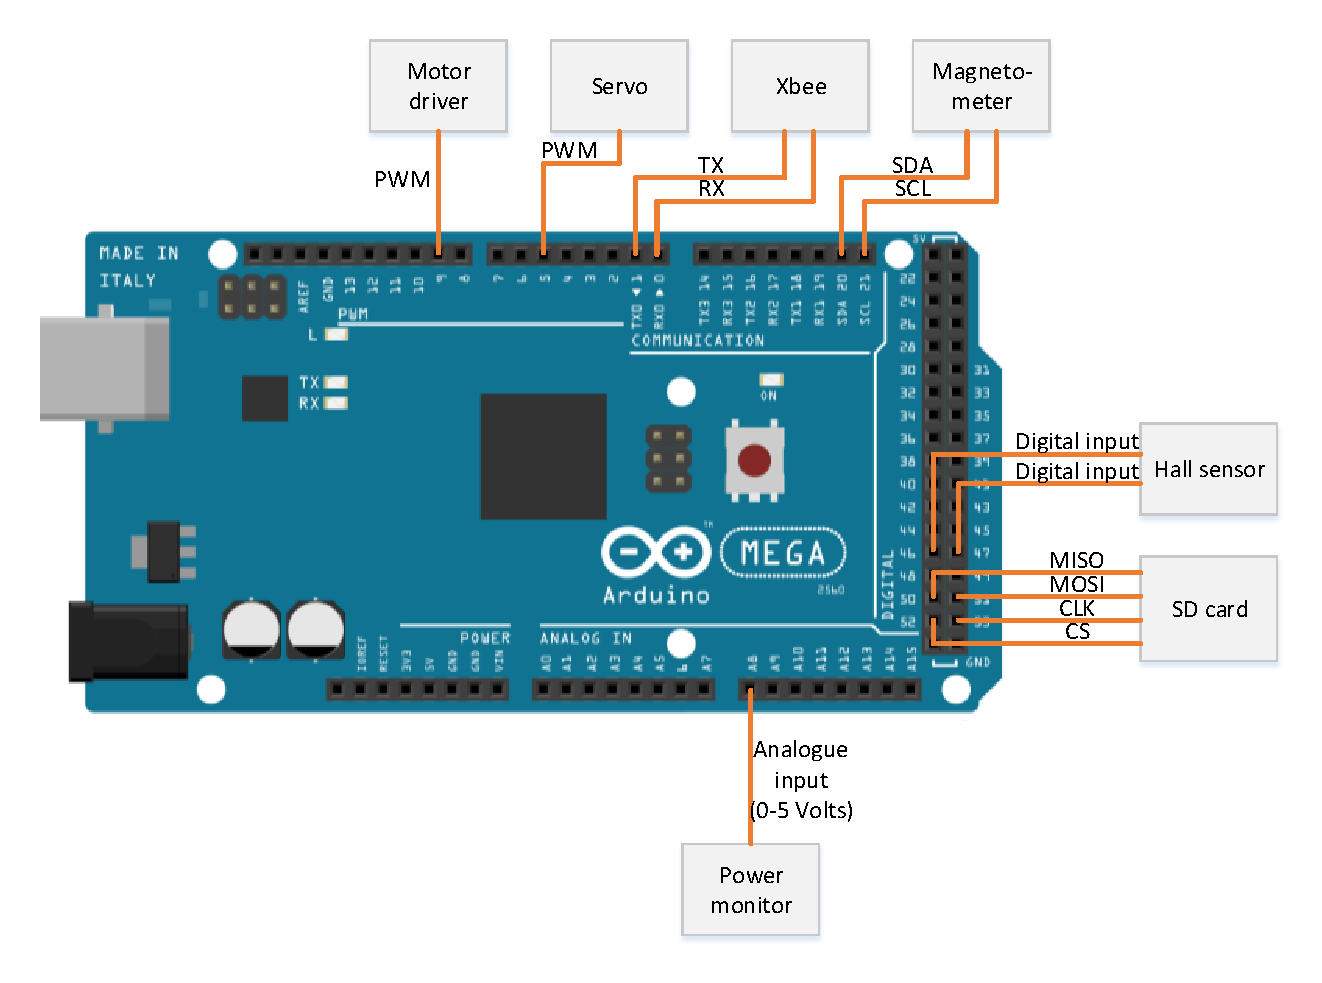
\includegraphics[scale=0.75]{figures/MegaSetup.pdf}
	\caption{Hey}
	\label{MegaSetup}
\end{figure}

The XBee module needs to connect to a serial port, and UART3 is chosen, as it makes it easiest to route the PCB traces. UART3 is located at pins 0 and 1. 

The SD-card needs an SPI connection, and must therefore be connected to the SPI pins 50, 51, 52 and 53. 

The "9 Degrees of Freedom"-board needs an $\text{I}^2\text{C}$ connection, and has to be connected to the Arduino's $\text{I}^2\text{C}$ pins 20 and 21. 

The PWM signals to the motor and servo can be set to any of the PWM pins. For easiest route, pin 9 for the motor and pin 5 for the servo is selected.

The input from the hall sensors will be measured by the input capture pins (ICP4 and ICP5), where timer4 and timer5 is connected to. On the Arduino board, it is pin 46 and 47.

Lastly will the voltage divider, for the power monitoring, be connected to a analogue pin, which will be pin A9.


As all hardware modules have now been assigned pins on the Arduino, the electrical requirements of each module will now be considered.

\subsection{Electrical considerations}

Before connecting hardware modules to the Arduino pins, signal voltage levels need to be considered:

\begin{itemize}
\item The Arduino itself uses 5V logic levels.\cite{MegaInfo}
\item The "9 Degrees of Freedom"-board needs 5V supply voltage and $\SI{3,3}{V}$ logic levels. \todo{source}
\item The servo needs $\SI{4,8}{V}$ - 6V supply voltage and 5V signal levels
\todo{source}
\item The SD-card needs $\SI{3,3}{V}$ supply voltage and signal levels, see \subsecref{SDcard}
\item The Hall sensors need $\SI{3,5}{V}$ - 24V supply, and a pull up resistor to define the logic level.
\todo{source}
\item The XBee module needs $\SI{3,3}{V}$ supply voltage and signal levels
\todo{source}
\end{itemize} 

The Arduino has regulated 5V and $\SI{3,3}{V}$ supply rails available, which will be used to power the respectable hardware modules. As the servo can potentially draw a lot of current, and overload the Arduino, it will be connected to a dedicated 5V voltage regulator, powered directly from the battery.

A low-dropout type is chosen, \textbf{L4941}, to make sure it works, even at low battery voltages. This regulator has a maximum dropout of 700mV at 1A current, meaning that it will work with battery voltages as low as $\SI{5,7}{V}$. \todo{datasheet} 

All one-directional connections from the Arduino to  $\SI{3,3}{V}$ logic level inputs will be connected to a HEF4050 CMOS buffer. This device can accept input voltages up to 15V, while supplied by as little as 3V supply voltage. This makes it ideal for uni-directional voltage level translation. \todo{datasheet}

One-directional connection from  $\SI{3,3}{V}$ logic level output to Arduino inputs will be connected directly, as $\SI{3,3}{V}$ is above the minimum high level threshold (Min $\text{V}_\text{IH}=\SI{0,6}\cdot \text{Vcc} = \SI{0,6}\cdot 5 = 3$V). \cite{Atmega}

As the $\text{I}^2\text{C}$ bus is using bi-directional connections, and needs to connect a $\SI{3,3}{V}$ system to a 5V system, this needs to be addressed as well. One solution could be running the bus at $\SI{3,3}{V}$, but this is unfortunately not possible, as the microcontroller needs at least $\SI{3,5}{V}$ as HIGH voltage, when in  $\text{I}^2\text{C}$ mode. \cite{Atmega}. The creators of $\text{I}^2\text{C}$, Philips, recommends solving this with two mosfets, see \figref{i2clevel}.

\begin{figure}[H]
	\centering
	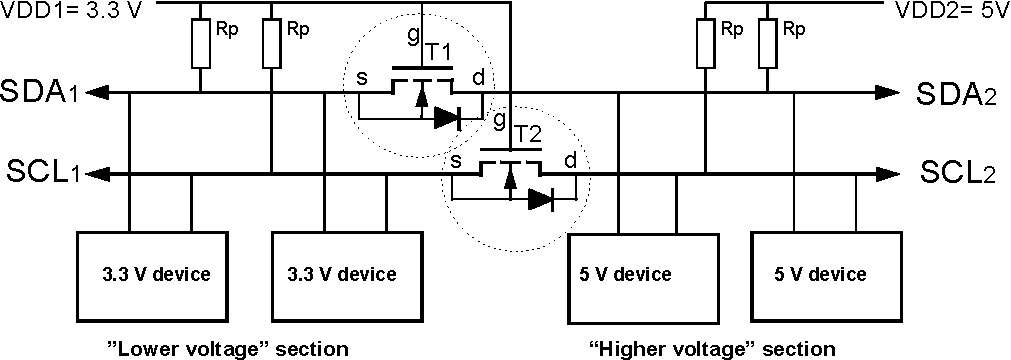
\includegraphics[scale=0.9]{figures/i2cLevel.pdf}
	\caption{$\text{I}^2\text{C}$ Voltage level translator. [source: Philips]}
	\label{i2clevel}
\end{figure}

\subsection{Voltage divider}

The power monitor need a voltage divider, see \secref{Hardwarechoice}. With a measurement interval on 0 to 5 volts in 1023 for the analogue pin on the Arduino, the voltage divider is need to design, to measure the whole interval for the battery pack. As the battery pack can have a voltage up to 8,4 volt \todo{Source, thomas}, the transfer constant for the voltage divider need to be smaller than 0,59 to measure the whole interval. The smaller the transfer constant, the bigger the interval is and the bigger will each step be. To make sure that there will not come a bigger voltage than 5 volts on the output from the voltage divider, the transfer constant is set to 0,5. This will give a maximum voltage into the voltage divider on 10 volts, before there will come more than 5 volts out on the output. To get a transfer constant on 0,5 the resistors in the voltage divider need to be the same, see \eqref{VolDivRes1} to \eqref{VolDivRes3}.

%\begin{flalign}
%\eq{R}{$R_1 = R_2$}\unit{\Omega}
%\label{VolDivRes1}
%\end{flalign}
\todo{Need to setup this equation, Niels please help me}

\begin{flalign}
\eq{V_{out}}{\frac{R}{R \cdot R} \cdot V_{in}}\unit{V}
\label{VolDivRes2}
\end{flalign}

\begin{flalign}
\eq{V_{out}}{\frac{1}{2} \cdot V_{in}}\unit{V} 
\label{VolDivRes3}
\end{flalign}

For the size of the resistors, the output impedance for the voltage divider have to be take into consideration. For the analogue pins on the Arduino, it is recommend to have a output impedance smaller than 10 $k\Omega$, or the it will begin to disturb the reading on the pin.
To make sure that is does not happen, the resistors in the voltage divider is set to the half of the maximum output impedance, 5 $k\Omega$. The closet resistor in the E96 series is 4,99 $k\Omega$, which will be use for both resistors. 

The final voltage divider circuit for the power monitor can be seen on \figref{VoltDivFigFinal}.
\begin{figure}[h!]
\centering
\begin{circuitikz}
\draw (0,2)
to[short,l=$V_{in}$] (1,2)
to[short] (2,2)
to[R=$R_1$] (2,0)
to[R=$R_2$] (2,-2);
\draw (2,-2) 
to[short] node[ground] {} (2,-3);
\draw (2,0)
to[short] (3,0)
to[short,l=$V_{out}$] (4,0);
\draw (2,0)
to[C=$C_1$] (0,0)
to[short] node[ground] {} (0,-1);
\end{circuitikz}
\caption{The implemented voltage divider} 
\label{VoltDivFigFinal}
\end{figure}

To filter the high frequency noise out, there is also implemented a 100 $nF$ capacitor in the voltage divider.

With all the hardware components physically implemented on the vehicle and to the microcontroller, there will be the brain of the system, there will be look at the implementation of the hardware components, in the Arduino software.

